%----------------Set Font Size & Layout----------------%
\documentclass[12pt, letterpaper, oneside]{article}
\usepackage{STYLE, amsfonts}
%---------------------Set Margins----------------------%
\usepackage[letterpaper, left=1in, right=1in,
top=1in, bottom=1in, bindingoffset=0mm]{geometry}
%-------------------Header & Footer-------------------%
\fancypagestyle{style1}{
\fancyhf{}
\chead{Title}
%\fancyhead[RO,LE]{Thesis Title}
\fancyfoot[C]{\thepage}
%\renewcommand{\headrulewidth}{0pt}
}
%\pagestyle{style1}
%------------------Title Page Settings------------------%
\title{The Title of the Paper\thanks{I thank Professor Chen and Hao-Che Hsu for useful comments and suggestions. All errors are my own.}}
\author{Your Name\footnote{Department of Economics, University of California-Irvine. E-mail: yourUCInetID@uci.edu. UCI-ID.}}
\date{2020}
%-------------------------Main-------------------------%
\begin{document}
%\setlength{\baselineskip}{16pt}
\doublespacing

\maketitle

\begin{abstract}
    Here is the abstract, a very brief summary of the whole paper. %\lipsum[1]
\end{abstract}

\noindent\textbf{Keywords:} Competition, pricing strategy\\

\noindent\textbf{JEL Code:} L10
\newpage

\section{Introduction}
\cite{chen2018} finds a strong network effect. Following the literature on numerically solving the problem \citep{chen2018}, I will simulate the model equilibrium in this paper.

I will do a case study and follow the instructions from a website \citep{web-io} to adopt a old but classic model from \cite{art}, an unpublished manuscript. But from another book, \cite{book-tirole} claims that there is bias in this approach.

\subsection{Industry Background}
Introduce the industry.

\section{Data}
Present data descriptive statistic. Show a table.

\section{Model}
Present your Econometric model.

\begin{theorem}[Theorem title]
    Theorem contents.
\end{theorem}
\begin{proof}
    Theorem Proofs.
\end{proof}

\subsection{Estimation}
Present your regression results.

\section{Conclusion}
Summarize your findings.

\bibliographystyle{JPE}
\bibliography{REFERENCE}

%----------------Syntax (Delete this part)---------------%
\begin{center}
    \textbf{\Large Useful \LaTeX \ Syntax}
    \noindent\rule{16cm}{0.4pt}
\end{center}

$\mathds{1}\{x>0\}=1$
\begin{figure}[h]
    \centering
    \caption{The function}
    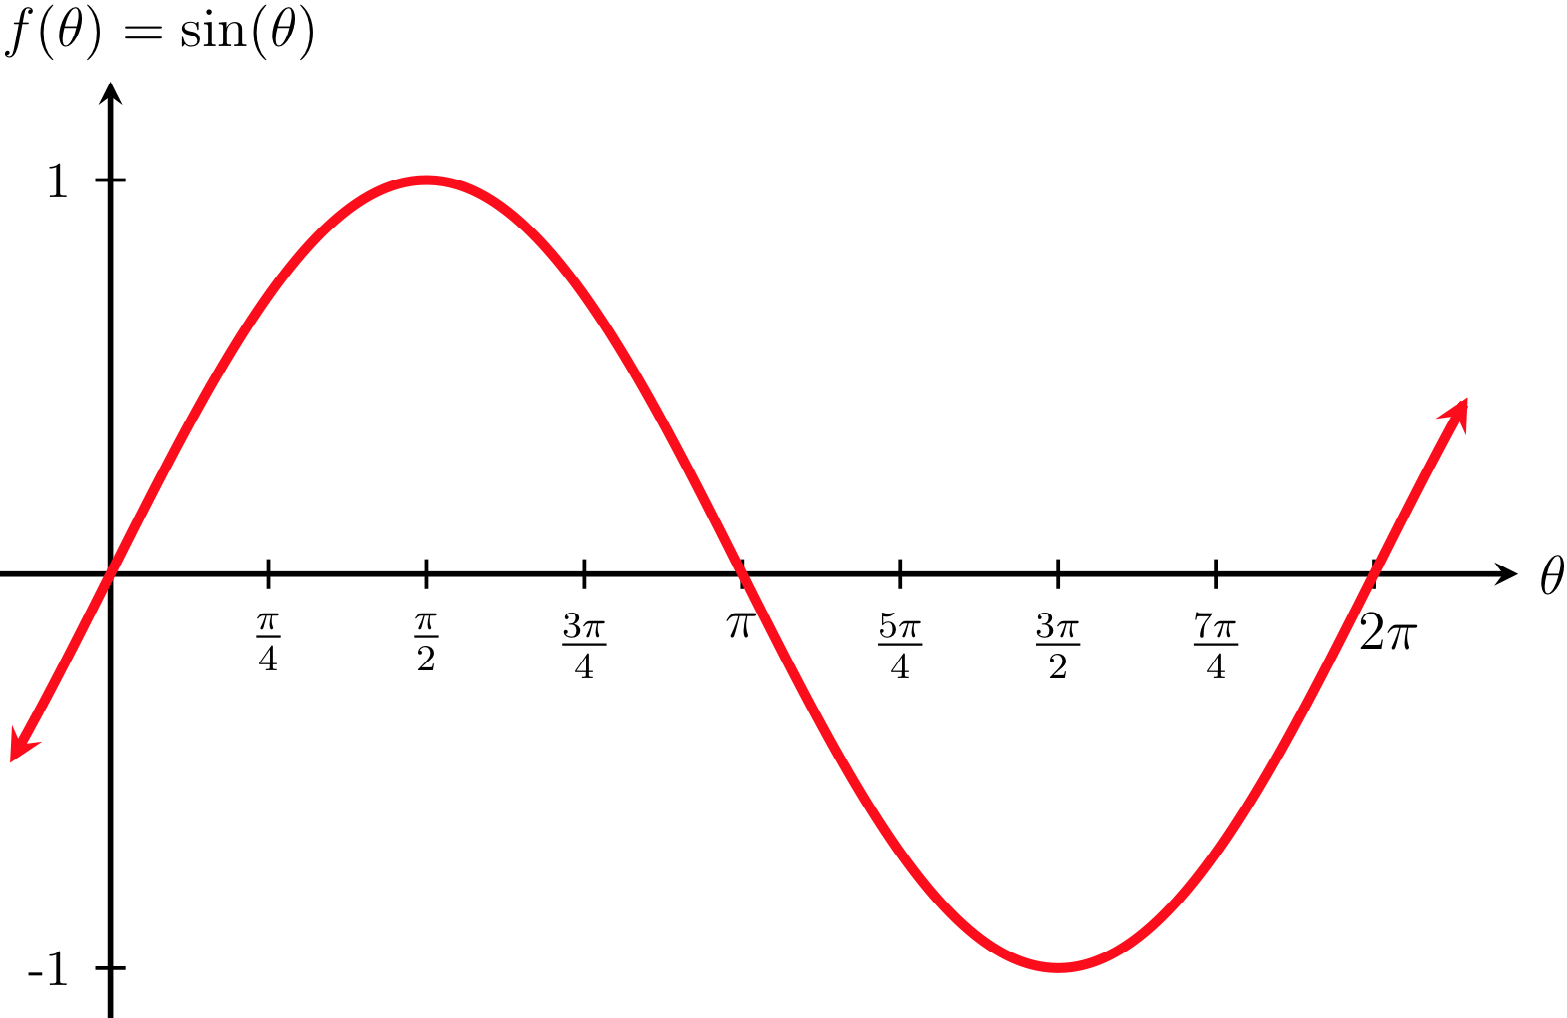
\includegraphics[scale=0.2]{graph.png}
\end{figure}

\vspace*{-1cm}

\begin{align}
    \mathcal{L}[\beta|(y_1,x_1),...,(y_n,x_n)]&=f[(y_1,x_1),...,(y_n,x_n)|\beta]\\
    &=\prod\limits_{i=1}^n\Big[\Phi(x_i'\beta)\Big]^{y_i}\Big[1-\Phi(x_i'\beta)\Big]^{1-y_i}
\end{align}

\begin{multicols}{2}
    \raggedcolumns
    \noindent \textbf{First Column:}\\
    contents in the first column.
    
    \columnbreak
    \noindent \textbf{Second Column:}\\
    contents in the second column.
\end{multicols}

\noindent $\overline{\text{MY TEXT}}$ \ \ $\underline{\text{MY TEXT}}$ \ \ $\underbrace{\text{MY TEXT}}_{\text{xyz}}$ \ \ $\underset{y\in\Gamma}{\max}$ \ \ $\widehat{\alpha\beta\gamma}$ \ \ $\widetilde{ABCD}$

\vspace*{0.1cm}

\begin{multicols}{3}
    \raggedcolumns
    $\begin{pmatrix}
    A & B &C \\
    D& E &F
    \end{pmatrix}$
    
    \columnbreak
    $\begin{bmatrix}
    A &B  &C \\
    D&  E& F
    \end{bmatrix}$
    
    \columnbreak
    $\begin{vmatrix}
    A &B  &C \\
    D&  E& F
    \end{vmatrix}$
\end{multicols}

$\bigstar$ A hyper link: \href{http://www.tablesgenerator.com}{\textcolor{blue}{Click to go to \textbf{LaTeX Tables Generator.}}}

\begin{itemize}
    \item first
    \item second
\end{itemize}

\begin{enumerate}
    \item one
    \item two
\end{enumerate}

\begin{align}
    VM_1&=\dfrac{R_x}{R_2+R_x}-\dfrac{R_3}{R_1+R_2} \\ \nonumber
    & \Longrightarrow  \hspace{0.2cm} R_1R_2VM_1 +R_2R_3VM1
\end{align}

$f_{R}(r)=\dfrac{dF}{dr}=\dfrac{r}{50}$, \quad
$\displaystyle E(r)=\int_{0}^{10}r \left( \dfrac{r}{50} \right)dr=\dfrac{r^{3}}{150}\biggr\rvert^{10}_{0}=\dfrac{1000}{150}=\dfrac{20}{3}$\\

\begin{equation}
    \bullet \ AR(1): \epsilon_t =(1-\rho L)x_t \Longrightarrow x_t=\rho x_{t-1}+\epsilon_t
\end{equation}

This is \textcolor{red}{color red}.

\definecolor{darkGreen}{HTML}{1e5c6c}
{\color{darkGreen}This is customized \textbf{color code}:1e5c6c\footnote{The color code can be obtained from Photoshop.}.}\\

\begin{flushleft}
    Display code:  \verb|sudo /usr/libexec/repair_packages --verify --standard-pkgs /|
\end{flushleft}

``This is the correct syntax for quotation mark!''

\newpage

{\fontsize{15}{11}\selectfont Customized size text, this is 15pt}

\vspace*{1cm}

$\text{ when }
\begin{cases}
    a(E)'=\infty, &\text{if $E=\bar{L}$} \\
    a(E)'=0, &\text{if $E=0$}
\end{cases}
$

\vspace*{1cm}

\begin{figure}[h!]
    \centering
    \begin{minipage}{0.72\textwidth}
        \begin{center}
            \captionsetup{justification=centering}
            \caption{Time Series of Fuel Cost Per Gallon for Selected Carriers During 2000 and 2015}
            \vspace*{-0.2cm}
            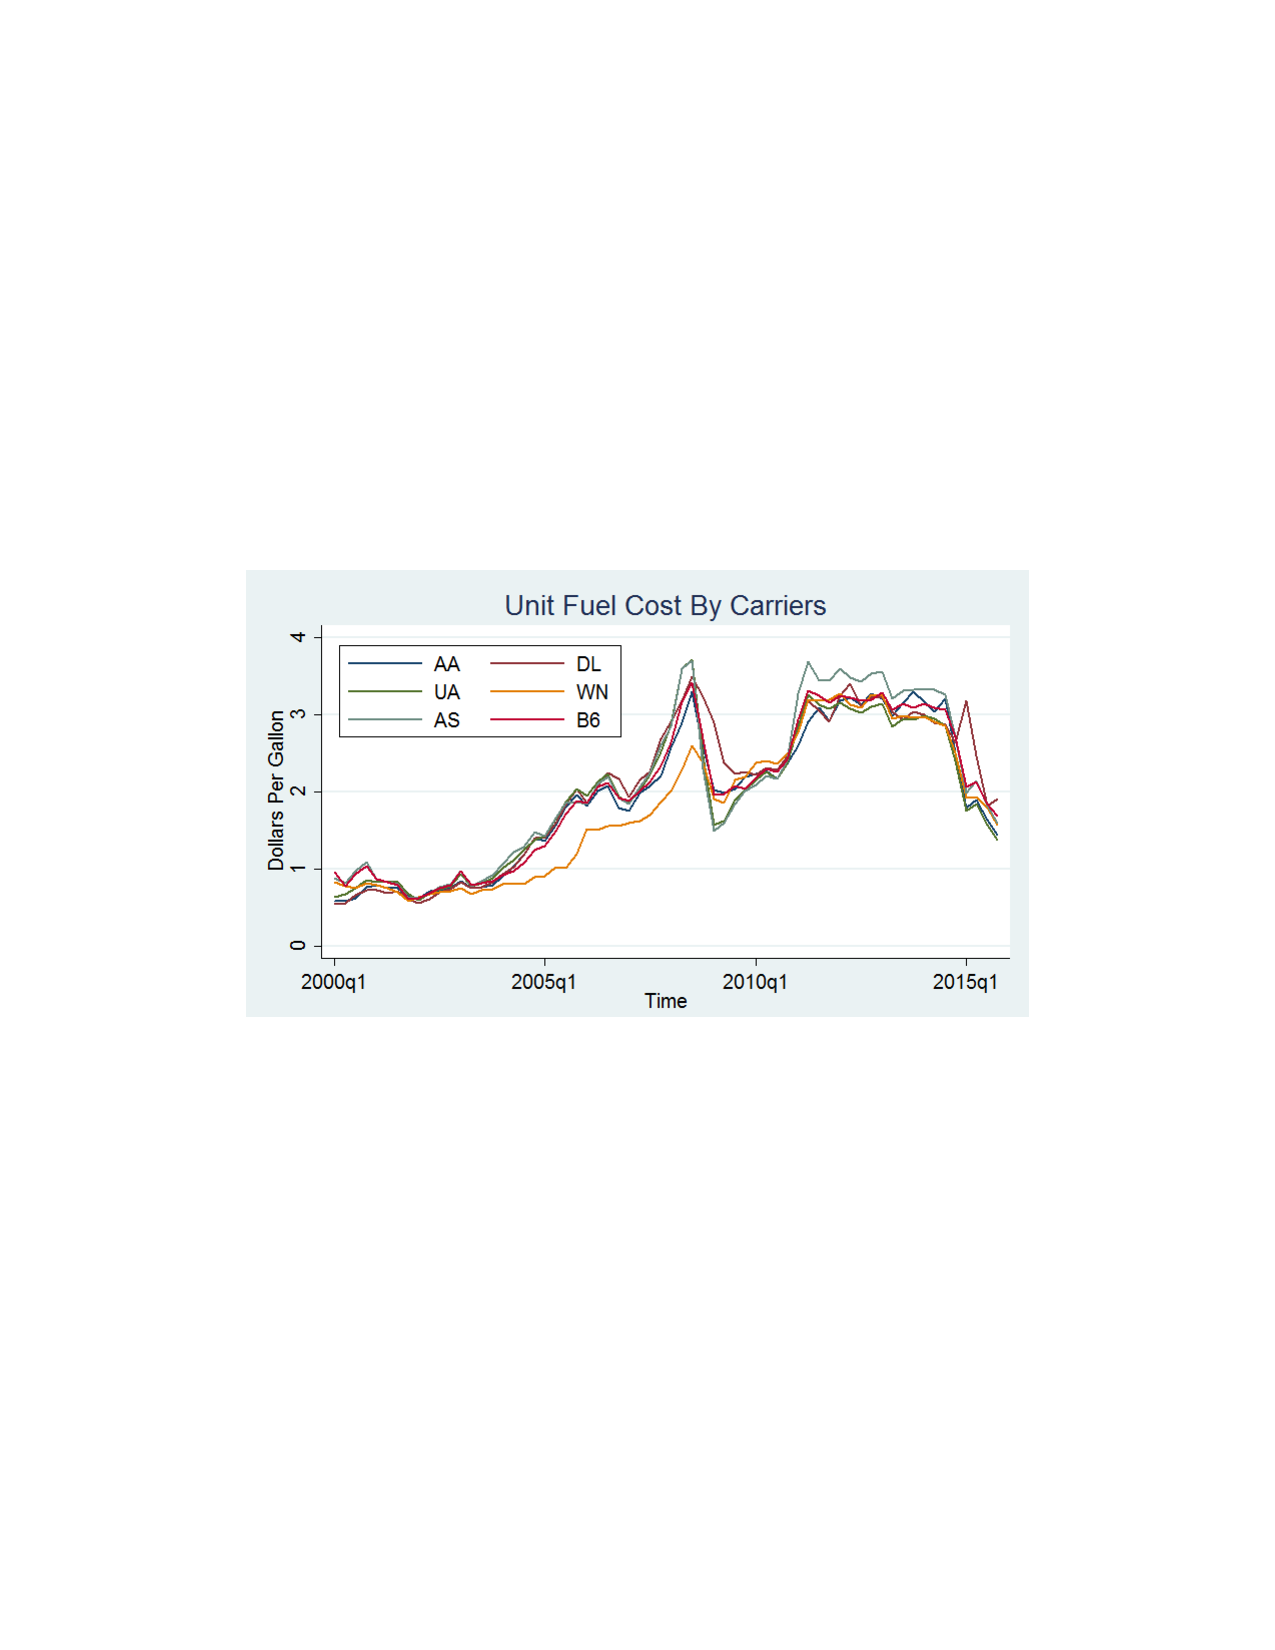
\includegraphics[scale=0.9]{photo.pdf}
        \end{center}
        \vspace*{-0.4cm}
        {\footnotesize  Source: Airline Origin and Destination Survey (D1B1), Bureau of Transportation Statistics (BTS). \par}
    \end{minipage}
\end{figure}

\renewcommand*\arraystretch{1.4} %stretch table (height)
\renewcommand{\tabcolsep}{14.3pt} %set table (width)
\begin{table}[h!]
    \fontsize{9.5}{11}\selectfont
    \centering
    \caption{Programming Languages}
    \begin{tabular}{ccccc}
        \hline
        & Python  & Java    & C    & Swift                                               \\ \hline
        Dfficulty & easy    & medium  & hard & \begin{tabular}[c]{@{}c@{}}very\\[-0.15cm] easy\end{tabular} \\
        OOP       & support & support & N/A  & support\\[0.15cm] \hline\hline
    \end{tabular}
    \hspace*{-0.58cm}
    \begin{minipage}{0.655\textwidth}
        \begin{tablenotes}
            \footnotesize
            \item A programming language is a formal language, which comprises a set of instructions that produce various kinds of output. Programming languages are used in computer programming to implement algorithms.
        \end{tablenotes}
    \end{minipage}
\end{table}
%----------------Syntax (Delete this part)---------------%

\end{document}